\documentclass[12pt, letterpaper]{article}
\usepackage{graphicx}
\usepackage[margin=1in]{geometry}
\usepackage{amsmath, amssymb, amsthm, mathrsfs}
\usepackage{fancyhdr}
\usepackage{tikz}
\usepackage{enumerate}
\usepackage{cancel}
\usetikzlibrary{positioning}
\usepackage[utf8]{inputenc}
\usepackage{xcolor}
\usepackage{framed}

\title{HW 1.3}
\author{Your Name}
\date{\today}

\pagestyle{fancy}
\renewcommand{\headrulewidth}{0pt}
\renewcommand{\footrulewidth}{0pt}
\fancyhf{}
\rhead{
    Zack Abdirashid\\
    2/3/26 \\
    MATH 405
}
\rfoot{Page \thepage}

\begin{document}

\paragraph{\underline{1.3} \\ \\} 

\textbf{6.} If a graph $G$ has $n$ vertices, all of which but one have odd degree, how many vertices of odd degree are there in $\overline{G}$, the complement of $G$? \\ \\
Since $1$ vertex is of even degree, there are $n-1$ vertices of odd degree, implying $n-1$ is an even number. $\therefore n$ must be odd. Let $a \in G$ such that deg($a$) = 2. \\

\begin{center}
    \begin{tikzpicture}[scale=1.5, every node/.style={circle,fill,minimum size=1px,inner sep=1.5pt}]
    \node[fill=none, inner sep=0pt] at (-1,1.5) {\underline{$G$}:};
    \node[label=90:$a$] (a) at (0,1) {};
    \node[label=180:$b$] (b) at (0,0) {};
    \node[label=0:$c$] (c) at (1,-0.5) {};
    \node[label=0:$d$] (d) at (2,-0.2) {};
    \node[label=45:$e$] (e) at (1.5,1.5) {};
    
    \draw (a) -- (b);
    \draw (a) -- (d);
    \draw (c) -- (e);
\end{tikzpicture}
\end{center}
\begin{center}
    * "complement" \Rightarrow \text{same \# of vertices but $\nexists$ edges from $G$ in $\overline{G}$.} \\
\end{center} 
\begin{center}
    \begin{tikzpicture}[scale=1.5, every node/.style={circle,fill,minimum size=1px,inner sep=1.5pt}]
    \node[fill=none, inner sep=0pt] at (-0.7,0.5) {$\Rightarrow$};
    \node[fill=none, inner sep=0pt] at (-1,1.5) {\underline{$\overline{G}$}:};
    \node[label=90:$a$] (a) at (0,1) {};
    \node[label=180:$b$] (b) at (0,0) {};
    \node[label=0:$c$] (c) at (1,-0.5) {};
    \node[label=0:$d$] (d) at (2,-0.2) {};
    \node[label=45:$e$] (e) at (1.5,1.5) {};
    
    \draw (a) -- (e);
    \draw (a) -- (c);
    \draw (b) -- (d);
\end{tikzpicture} \\
\Rightarrow \ \boxed{\text{$n-1$ vertices of odd degree}}
\end{center}



\textbf{10.} There used to be 26 football teams in the National Football League (NFL) with 13 teams in each of two conferences. An NFL guideline said that each team's 14-game schedule should include exactly 11 games against teams in its own conference and three games against teams in the other conference. By considering the right part of a graph model of this scheduling problem, show that this guideline can not be satisfied! 
\begin{center}
    \begin{framed}
        Let $C$ be a graph of one of the conferences containing $13$ teams. Representing teams as vertices and edges as games between two teams, there are $13$ (odd) vertices each of degree 11 (odd) in $C$. But, the \# of vertices of odd degree in any graph $G$ must be even. $\therefore$ it is impossible for $13$ teams to play $11$ games each against each other which does not satisfy the guideline.
    \end{framed}
\end{center}

\textbf{16.} Determine whether the following graphs are bipartite. If so, give the partition into left and right vertices. \\
\indent{} \textbf{(a)} 
\begin{center}
    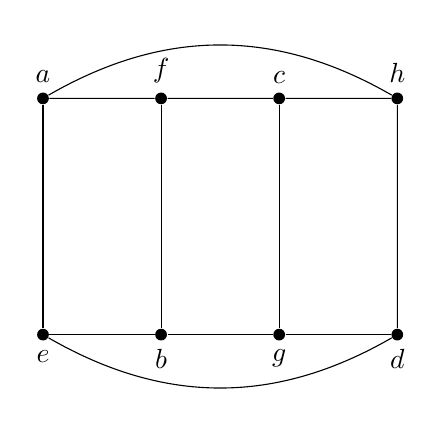
\begin{tikzpicture}[scale=1.5, every node/.style={circle,fill,minimum size=1px,inner sep=1.5pt}]
    % Top vertices
    \node[label=90:$a$] (a) at (0,2) {};
    \node[label=90:$f$] (f) at (1,2) {};
    \node[label=90:$c$] (c) at (2,2) {};
    \node[label=90:$h$] (h) at (3,2) {};
    
    % Bottom vertices
    \node[label=270:$e$] (e) at (0,0) {};
    \node[label=270:$b$] (b) at (1,0) {};
    \node[label=270:$g$] (g) at (2,0) {};
    \node[label=270:$d$] (d) at (3,0) {};
    
    % Vertical edges
    \draw (a) -- (e);
    \draw (f) -- (b);
    \draw (c) -- (g);
    \draw (h) -- (d);
    \draw (a) -- (f);
    \draw(f) -- (c);
    \draw(c) -- (h);
    \draw(e) -- (b);
    \draw(b) -- (g);
    \draw(g) -- (d);
    % Top arc
    \draw (a) to[bend left=30] (h); 
    
    % Bottom arc
    \draw (e) to[bend right=30] (d);
\end{tikzpicture}
\end{center}
\begin{center}
Select vertex $a$ and put it on the left.  \\
* If $a$ has a path of odd length to some vertex $x$, put $x$ on the right. Otherwise, put $x$ on the left. \\
* If two adjacent vertices $x$ and $y$ are on the same side, the graph is \underline{not} bipartite.
\end{center}

\begin{center}
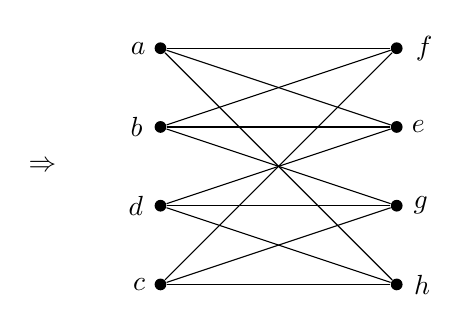
\begin{tikzpicture}[every node/.style={circle,fill,minimum size=1px,inner sep=1.5pt}]
    \node[fill=none, inner sep=0pt] at (-1.5,1.5) {$\Rightarrow$};
    \node[label=180:$a$] (a) at (0,3) {};
    \node[label=180:$b$] (b) at (0,2) {};
    \node[label=180:$d$] (d) at (0,1) {};
    \node[label=180:$c$] (c) at (0,0) {};
    
    \node[label=0:$f$] (f) at (3,3) {};
    \node[label=0:$e$] (e) at (3,2) {};
    \node[label=0:$g$] (g) at (3,1) {};
    \node[label=0:$h$] (h) at (3,0) {};
    
    \draw (a) -- (f);
    \draw (a) -- (e);
    \draw (a) -- (h);
    \draw (b) -- (f);
    \draw (b) -- (e);
    \draw (b) -- (g);
    \draw (d) -- (e);
    \draw (d) -- (g);
    \draw (d) -- (h);
    \draw(c) -- (f);
    \draw(c) -- (g);
    \draw(c) -- (h);
\end{tikzpicture} \\
\Rightarrow \ \boxed{\text{This graph is bipartite}}.
\end{center} 
\hspace{0.5cm} 
\textbf{(b)} 
\begin{center}
    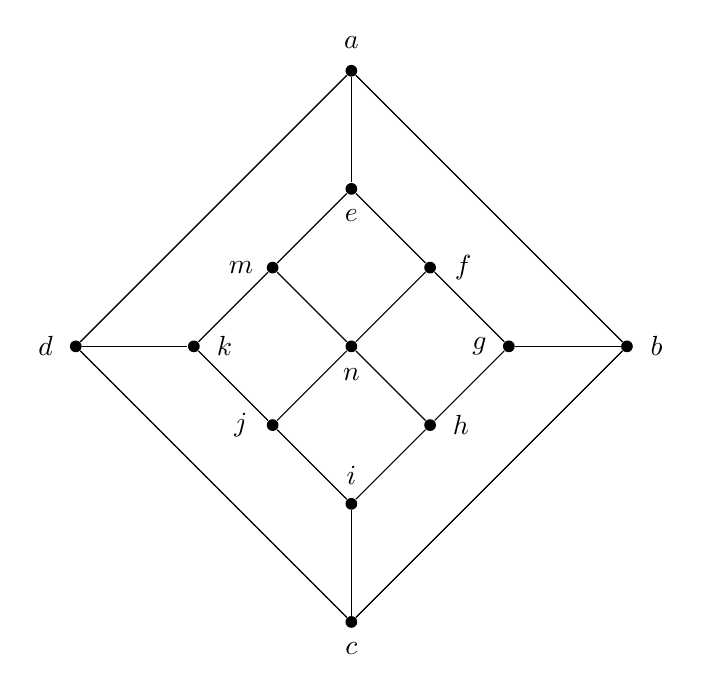
\begin{tikzpicture}[
    every node/.style={circle, fill=black, inner sep=1.5pt},
    label distance=2pt
]

    % Define coordinates
    % Central vertex
    \node (n) at (0,0) [label=below:$n$] {};

    % Inner ring vertices
    \node (m) at (-1,1) [label=left:$m$] {};
    \node (f) at (1,1) [label=right:$f$] {};
    \node (h) at (1,-1) [label=right:$h$] {};
    \node (j) at (-1,-1) [label=left:$j$] {};

    % Middle ring vertices
    \node (e) at (0,2) [label=below:$e$] {};
    \node (g) at (2,0) [label=left:$g$] {};
    \node (i) at (0,-2) [label=above:$i$] {};
    \node (k) at (-2,0) [label=right:$k$] {};

    % Outer ring vertices
    \node (a) at (0,3.5) [label=above:$a$] {};
    \node (b) at (3.5,0) [label=right:$b$] {};
    \node (c) at (0,-3.5) [label=below:$c$] {};
    \node (d) at (-3.5,0) [label=left:$d$] {};

    % Connect Inner Ring to Center
    \draw (n) -- (m);
    \draw (n) -- (f);
    \draw (n) -- (h);
    \draw (n) -- (j);

    % Connect Inner Ring to Middle Ring
    \draw (m) -- (e);
    \draw (f) -- (e);
    \draw (f) -- (g);
    \draw (h) -- (g);
    \draw (h) -- (i);
    \draw (j) -- (i);
    \draw (j) -- (k);
    \draw (m) -- (k);

    % Connect Middle Ring to Outer Ring
    \draw (e) -- (a);
    \draw (g) -- (b);
    \draw (i) -- (c);
    \draw (k) -- (d);

    % Outer Boundary connections
    \draw (a) -- (b) -- (c) -- (d) -- (a);
    
    % Diagonal outer connections
    \draw (a) -- (d);
    \draw (a) -- (b);
    \draw (c) -- (d);
    \draw (c) -- (b);
\end{tikzpicture}
\end{center}
\begin{center}
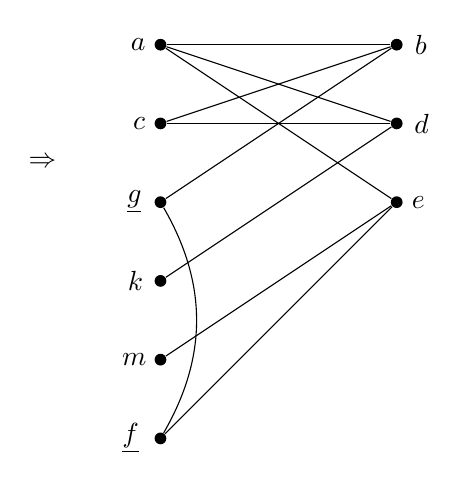
\begin{tikzpicture}[every node/.style={circle,fill,minimum size=1px,inner sep=1.5pt}]
    \node[fill=none, inner sep=0pt] at (-1.5,1.5) {$\Rightarrow$};
    \node[label=180:$a$] (a) at (0,3) {};
    \node[label=180:$c$] (c) at (0,2) {};
    \node[label=180:$\underline{g}$] (g) at (0,1) {};
    \node[label=180:$k$] (k) at (0,0) {};
    \node[label=180:$m$] (m) at (0,-1) {};
    \node[label=180:$\underline{f}$] (f) at (0,-2) {};
    
    \node[label=0:$b$] (b) at (3,3) {};
    \node[label=0:$d$] (d) at (3,2) {};
    \node[label=0:$e$] (e) at (3,1) {};
    
    \draw (a) -- (b);
    \draw (a) -- (d);
    \draw (a) -- (e);
    \draw (b) -- (c);
    \draw (b) -- (g);
    \draw (c) -- (d);
    \draw (g) to[bend left=30] (f);
    \draw (k) -- (d);
    \draw (m) -- (e);
    \draw(e) -- (f);
\end{tikzpicture} \\
\Rightarrow \ \boxed{\text{This graph is \underline{not} bipartite}}.
\end{center} 
\end{document}